Mobile Geräte sind heutzutage ein sehr großer Teil unseres Tagesablaufs. Durchschnittlich verbringen wir 3:54 Stunden pro Tag an mobilen Geräten (hier bezogen aus Bürger der USA). Die meiste Zeit hiervon wird in Apps (ca. 90\%). \footnote{\url{https://www.emarketer.com/content/us-time-spent-with-mobile-2019}, zuletzt aufgerufen: 26.02.2021} 
Laut Cisco wird dieser Markt sich jedoch nicht nur auf Industrieländer beruhen, sondern bis 2023 sollen weltweit 71\% der Bevölkerung mobile Konnektivität haben. \cite{cisco2020}
Diese Entwicklung forcierte viele Firmen immer mehr ihre Anwendungen auch \textit{mobile ready} zu gestalten. Dies kann man bspw. deutlich bei der Anpassung vieler Webseiten an Mobile Seiten- und Größenverhältnisse oder auch dem Anbieten von \textit{Apps}, welche bereits für Desktop o.ä. verfügbar waren, erkennen. \\

Daher ist es für die Wirtschaft und Entwicklung gleichermaßen wichtig sich ständig weiterzuentwickeln und sich nicht auf (Kosten-) ineffiziente Entwicklungsprozesse auszuruhen. Dabei bieten jährliche, wenn nicht sogar halbjährliche Design- und Performanceänderungen von den Geräten selbst oder der Betriebssysteme Herausforderungen an die mobilen Anwendungen und gleichzeitig an deren Programmierumgebung. Trotz einer riesigen Auswahl an \textit{Apps} lassen sich diese allgemein in drei Kategorien eingliedern: Plattformspezifische Native Anwendungen, Adaptive Webanwendungen und Plattformübergreifende Native Anwendungen.

\subsubsection{Plattformspezifische native Anwendungen}
Plattformspezifische oder auch native Anwendungen sind Programme, welche auf eine gewisse Plattform abzielen und in einer der davon unterstützen Programmiersprachen geschrieben wurden. Da diese Art der (mobilen) Anwendung mit plattformspezifischen \textit{Software Development Kits (SDK)} und \textit{Frameworks} entwickelt wird, ist diese Anwendung an eine Plattform gebunden. \\
Dies bringt zum einen natürlich Vorteile wie allgemein best mögliche Performance auf der jeweiligen Plattform und direkt vom Hersteller unterstützte Entwicklungsumgebungen/SDKs.
Zudem lassen sich plattformspezifische Fähigkeiten oder Einstellungen nutzen - beispielsweise mehrere Kameras oder \textit{Global Positioning System (GPS)}.

Gleichzeitig beschränkt man sich aber logischerweise auf eine Plattform und deckt mit einer Anwendung nur einen Teil des gesamten Marktes. Dies bringt im Vergleich zu den anderen Möglichkeiten einen deutlich erhöhten Entwicklungs- und Wartungsaufwand mit sich, da für andere Plattformen Programmcode nicht übernommen werden kann. Zusätzlich benötigen Entwickler spezifische Kompetenzen für beide Plattform und Entwicklungsumgebungen. \\

Zwei der am weitesten verbreiteten Plattformen sind Android von Google und iOS von Apple. Anwendungen für Android können in Kotlin oder Java als Programmiersprache beispielsweise in dem \textit{integrated development environment (IDE)} von Google Android Studio entwickelt werden. Für iOS wird hingegen mit Objective-C und Swift als Programmiersprache primär in der IDE XCode entwickelt.

Beide bieten jeweils Plattform eigene Services an, beispielsweise das direkte Veröffentlichen in den jeweiligen Appstore \cite{fentaw2020}
\subsubsection{Adaptive Webanwendungen}



\subsubsection{Plattformübergreifende Anwendungen}

\subsubsection{Flutter}
Flutter ist eine open-source SDK entwickelt von Google und ist geschrieben in C, C++ und Dart.
Flutter erlaubt es Anwendungen für Android, iOS, Web und Desktop basierend auf einem Code zu erstellen und ist zudem die primäre Methode für Google Fuchsia, Googles Betriebssystem.\footnote{Quelle: \url{https://fuchsia.dev/}}
Flutter verwendet \href{https://skia.org/}{Skia} als 2D Grafikbibliothek, welche auch von Chrome, Firefox und Android verwendet wird. Zudem basiert Flutter auf der Dart Plattform welche das Compilieren auf 32-bit und 64-bit ARM Prozessoren, auf Intel x64 Prozessoren und in JavaScript ermöglicht (siehe Abbildung \ref{fig:dart_plattform}). 

Während der Entwicklung werden Flutter Apps in einer Virtuellen Maschine (VM) gestartet, welche \textit{stateful hot reload} ermöglicht - bei Änderungen muss die App also nicht komplett neu kompiliert werden. Wird die App nun veröffentlicht, wird sie in die Maschinencode der beschriebenen Plattformen übersetzt.
\\

\begin{figure}[tbt]
	\begin{center}
		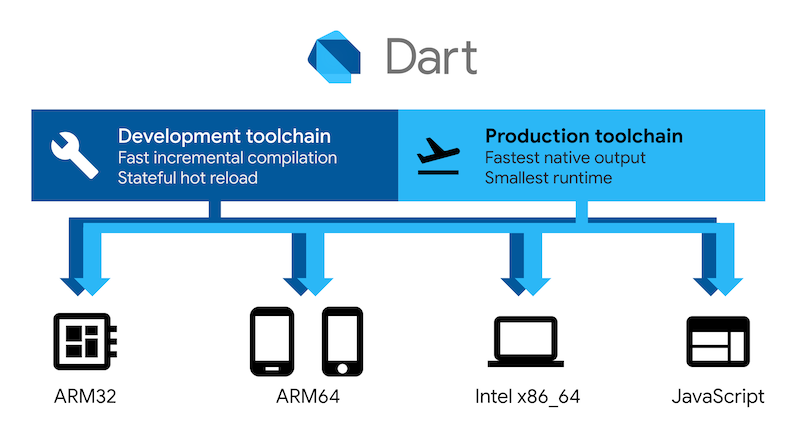
\includegraphics[scale=0.45]{images/dart-diagram.png}
	\end{center}
	\caption{Kompatibilität der Dart Plattform \protect \footnotemark}
	\label{fig:dart_plattform}
\end{figure}
\footnotetext{Quelle: \url{https://github.com/flutter/flutter}}

\paragraph{Architektur}
\begin{displayquote}
	Flutter is designed as an extensible, layered system. It exists as a series of independent libraries that each depend on the underlying layer. No layer has privileged access to the layer below, and every part of the framework level is designed to be optional and replaceable.\footnote{\url{https://flutter.dev/docs/resources/architectural-overview}}
\end{displayquote}

Grundlegend ist das Framework in drei Prozesseinheiten gegliedert. Diese bestehen wiederum jeweils aus, für sie charakteristischen APIs und Bibliotheken:

\begin{itemize}
	\item \textit{Flutter embedder}: Der Einstiegspunkt in die jeweilige Plattform. Er koordiniert Zugriffe auf Services des Betriebssystems; er ist also zuständig für bspw. die Kommunikation mit dem Input Method Editor (IME) und den Lifecycle Events der App. Daher ist der Embedder in der, von der Plattform unterstützten Programmiersprache geschrieben: derzeit wird Java und C++ für Android, Objective-C/Objective-C++ für iOS und macOS, und C++ für Windows und Linux verwendet.
	\item \textit{Flutter Engine}: Der Kern von Flutter, geschrieben hauptsächlich in C und C++, ist die \textit{low-level} Implementierung der Flutter Kern Programmierschnittstelle (API). Daher ist sie zuständig für das graphische Darstellen (Rasterisierung) des Codes sobald ein neuer \textit{Frame} angezeigt werden muss. Im Flutter Framework wird die \textit{Engine} als dart:ui Bibliothek offengelegt - der zugrundeliegende C++ Code wird in Dart Klassen eingefügt. 
	\item \textit{Flutter Framework}: Das Framework, mit welchem der Entwickler schlussendlich meistens arbeiten wird. Es ist in Dart geschrieben und bietet sogenannte \textit{Layer} für Animationen, Layout und Widgets. Widgets werden von Flutter als Einheit der Komposition von Benutzeroberflächen verwendet und sind als einzelne Bausteine zu verstehen, welche zusammengefügt ein Objekt oder sogar einen kompletten Bildschirm ergeben.
\end{itemize}

Bei der Entwicklung mit Flutter wird ein Baum von Widgets erzeugt, welcher als Bauplan der Applikation angesehen werden kann. Nach diesem Plan wird mithilfe von States der einzelnen Widgets schlussendlich das User Interface (UI) gerendert.\cite{flutter2021}

\begin{figure}[tbt]
	\begin{center}
		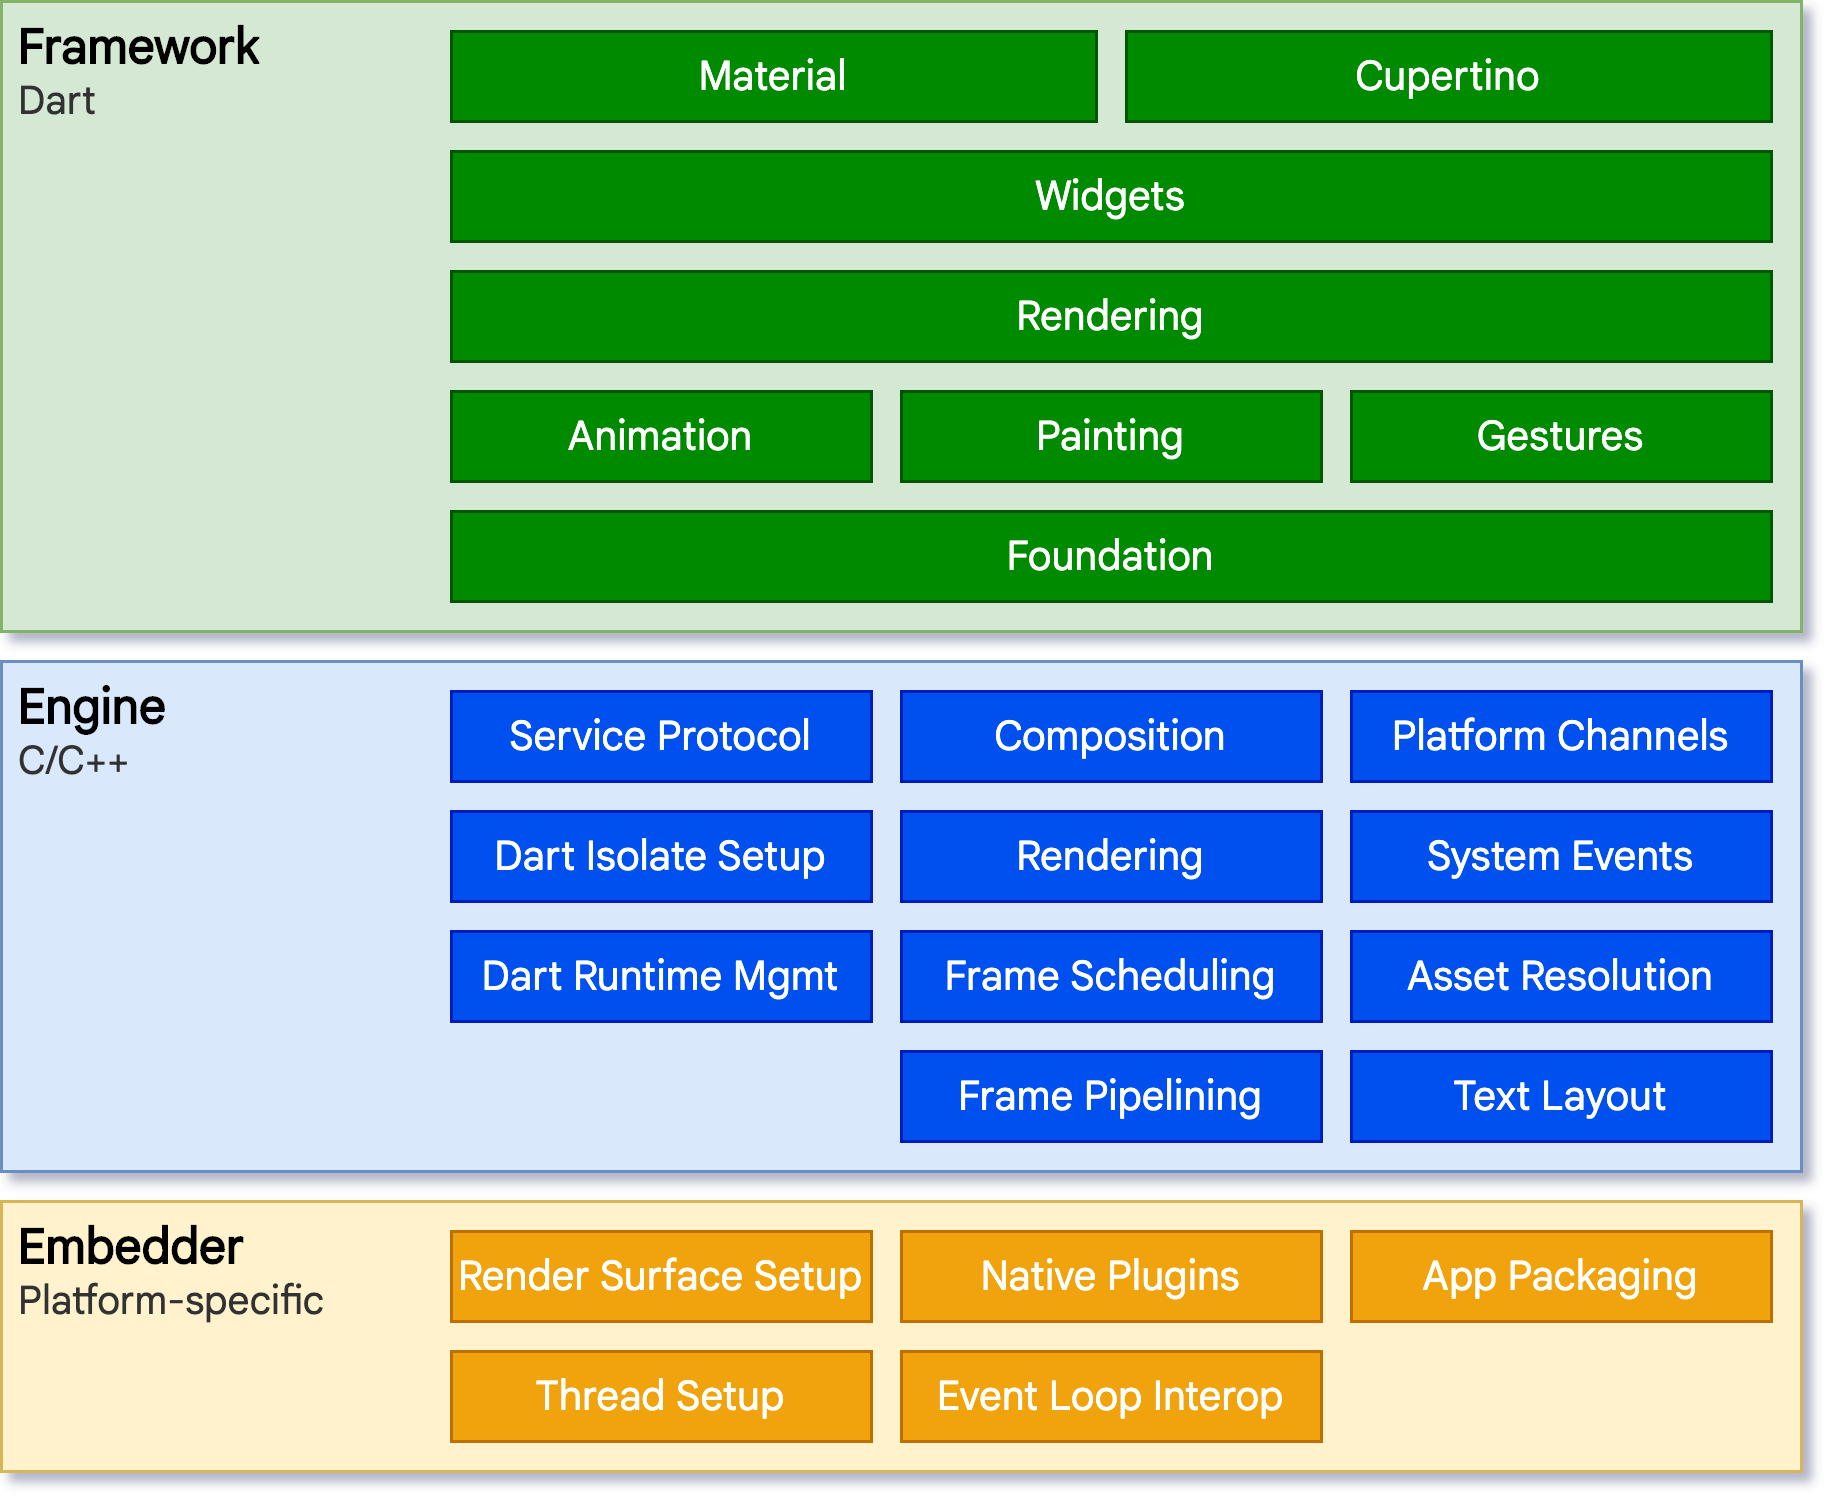
\includegraphics[scale=0.25]{images/flutter_architektur.png}
	\end{center}
	\caption{Bibliotheken und Ebenen der Flutter Plattform \protect \footnotemark}
	\label{fig:flutter_plattform}
\end{figure}
\footnotetext{Quelle: \url{https://github.com/flutter/flutter}}








\paragraph{Widgets}
\paragraph{States}

\subsubsection{React Native}


